% !TEX root = ../thesis.tex

\chapter{Data analysis}\label{sec:data_analysis}

\section{A statistical framework for tracking data}

The modern imaging methods described in chapter \ref{sec:introduction} have made possible to track simultaneously multiple particles at high spatiotemporal resolution. Single-particle tracking can then be used to reconstruct thousands of particle trajectories. To extract meaningful insights from this huge amount of data, we need a modelling and statistical framework.

In this chapter we will present data analysis techniques to reconstruct the dynamics of amyloid-β aggregates. As explained in section \ref{sec:alzheimer}, the uncontrolled formation of Aβ plaques in the brain tissue is thought to be a cause of Alzheimer's disease. What we would like to understand is how cells react to an excessive concentration of Aβ. How do they try to dispose of this dangerous products? We hypothesise that the cell transports and actively treats Aβ molecules for disposal in a well defined system. We tried to reconstruct the motion of Aβ molecules inside the cell to realise which route they follow and how they are treated. That said, the statistical methods described in the following aim to provide a general framework to extract dynamical parameters of particles at cell scale.

The data presented here was provided by the Molecular Neuroscience Group at the University of Cambridge, \tsc{UK}. It consists into trajectory fragments of Aβ-42 aggregates artificially injected in \tsc{HEK 293T} cells and captured via fast \tsc{SIM} (in \tsc{2d}) at a frequency of \SI{8}{\hertz}. The trajectories were reconstructed from imaging data using the TrackMate software.\mcite{trackmate}

\section{Model and methods}

At the microscopic level, the motion of the molecules can be described by Langevin's equation. In the case of biological processes we are interested in, the Langevin dynamics can be considered in its large friction limit (Smoluchowski's equation)\mcite{hoze2012, hoze2014}
\begin{equation} \label{eq:smoluchowski}
 \dot{\bm{x}} = \frac{\bm{F}(\bm{x})}{\gamma} + \sqrt{2D} \dot{\bm{w}}
\end{equation}
where $\bm{F}(\bm{x})$ is the drift force exerted on the particle at position $\bm{x}$, $\gamma$ is the friction coefficient, $D$ is the diffusion coefficient and $\bm{w}(t)$ is a two-dimensional Wiener process. At this scale, it makes sense to consider the diffusion to be mainly due to thermal agitation so that it can be considered isotropic.

However, it is not possible to directly recover the microscopic model from the \tsc{spt} data, since we miss information about the local behaviour both in space (such as the presence of microscopic obstacles undetected by the imaging device) and time (such as thermal fluctuations much faster than the acquisition timescale).\mcite{hoze2017, holcman2015} We can still build a coarse-grained model,\mcite{hoze2012, hoze2014} transforming eq. \ref{eq:smoluchowski} into the effective stochastic equation
\begin{equation} \label{eq:effective}
 \dot{\bm{x}} = \bm{a}(\bm{x}) + \sqrt{2}\bm{B} \dot{\bm{w}}
\end{equation}
where $\bm{a}(\bm{x})$ is the effective velocity field and $\bm{D} \equiv \bm{B}^T\bm{B}$ is the effective diffusion tensor. It must be noted that, in principle, the effective diffusion coefficient may not be isotropic since it takes into account the local microscopic features (e.g. obstacles). On the other hand, actual analysis of the data show that anisotropic components are negligible: in the following, the diffusion tensor is reduced for simplicity to a scalar coefficient by averaging on the diagonal entries. Moreover, the velocity field is assumed time invariant in the relatively short time window spanned by the \tsc{spt} data (30--60 s).

\begin{figure}
    \begin{adjustwidth*}{}{-46mm}
      \includegraphics[width=186mm]{spt/2_field.eps}%
      {{\phantomsubcaption{}\label{fig:vf_original}}%
      {\phantomsubcaption{}\label{fig:vf_smooth}}%
      {\phantomsubcaption{}\label{fig:vf_cdr}}}%
      \caption{Velocity field obtained from the \tsc{SPT} data using bins of size \SI{250}{\nano\metre}. \subref{fig:vf_original}\enskip original velocity field, \subref{fig:vf_smooth}\enskip velocity field after smoothening. \subref{fig:vf_cdr}\enskip regions of coherent motion obtained by clustering the smoothened velocity field. The angular distance threshold was set to \SI{0.08}{} and clusters smaller than 10 bins were discarded. The area color indicates the mean angle of the velocity among the cluster.\label{fig:vf}}
  \end{adjustwidth*}
\end{figure}


\subsection{Diffusion and velocity field estimation}

To estimate the dynamical parameters of eq. \ref{eq:effective} a statistical analysis is needed. We follow the approach demonstrated in \cite{hoze2012,hoze2014,hoze2017,holcman2015} by partitioning the data in a square grid with fixed bin size. The velocity field and diffusion coefficients are considered constant in each bin.
If the acquisition time interval is sufficiently small, the process described by eq. \ref{eq:effective} can be discretised following a forward Euler scheme:
\begin{equation}
 \bm{x}_{t+1} - \bm{x}_{t} = \bm{a}_{\Delta t}(\bm{x}_t) \Delta t + \sqrt{2\Delta t\bm{D}_{\Delta t}(\bm{x}_t)}  \bm{\eta}_t
\end{equation}
where $\Delta t$ is the acquisition time interval.

Then, the trajectory step $\Delta\bm{x}_t \equiv \bm{x}_{t+1} - \bm{x}_t$ starting in bin $B$ is a normally distributed random variable with mean $\bm{a}(\bm{x}_B)$ and variance $2D(\bm{x}_B)\Delta t$ where $\bm{x}_B$ is the center of the bin. The velocity field and diffusion tensor can thus be recovered by computing the empirical estimate of the moments:
\begin{align}
 \bm{a}_{\Delta t}(\bm{x}_B) & = \frac{1}{\Delta t} \mathbb{E}_B\left[\Delta \bm{x}\right]                                                   \\
 \bm{D}_{\Delta t}(\bm{x}_B) & = \frac{1}{2\Delta t} \left( \mathbb{E}_B\left[\Delta \bm{x}^2\right] - \mathbb{E}_B[\Delta \bm{x}]^2 \right)
\end{align}
where the expected value is taken on the bin. Notice that the $\bm{a}_{\Delta t}$ and $\bm{D}_{\Delta t}$ are not the same of those of eq. \ref{eq:effective}, as they depend on the acquisition interval $\Delta t$. In fact, we may recover the coefficients of the continuous process only in the limit $\Delta t \to 0$. To avoid a too cluttered notation, we will drop the $\Delta t$ index in the following and assume it implicitly.


\subsection{Field smoothening}\label{sec:smoothening}

To perform analysis and simulations we often need a smooth representation of the velocity or diffusion field, providing estimates also for bins with few—or missing—data. To solve this problem, a convolution with variable kernel is applied on the field. Denoting by $n_B$ the number of datapoints inside bin $B$, the smoothened field $\tilde{\bm{a}}$ is obtained as
\begin{equation} \label{eq:convolution}
 \bm{\tilde{a}}(\bm{x}_B) = (k \ast a)(\bm{x}_B) \equiv \frac{\displaystyle \sum_{S \in \Gamma(B)} n_S \bm{a}(\bm{x}_S)}{\displaystyle \sum_{S' \in \Gamma(B)} n_{S'}}
\end{equation}
where $\Gamma(B)$ is the Moore neighbourhood of $B$.

Explicitly, representing bins with their grid site indices, the kernel matrix $K(i, j)$ centered in the bin $i, j$ is:
\begin{equation}
 K(i, j) = \frac{1}{\displaystyle \sum_{k = i-1}^{i+1}\sum_{l = j-1}^{j+1} n_{k,l}}
 \begin{bmatrix}
  n_{i-1,j-1} & n_{i-1, j} & n_{i-1, j+1} \\
  n_{i,j-1}   & n_{i, j}   & n_{i, j+1}   \\
  n_{i+1,j-1} & n_{i+1, j} & n_{i+1, j+1}
 \end{bmatrix}
\end{equation}
Finally, bins such that the total number of samples in their Moore neighbourhood is lower than a threshold are excluded from the analysis. A comparison between the velocity field before and after the smoothening is visible in \cref{fig:vf_original,fig:vf_smooth}.

This approach can be interpreted in terms of Bayesian inference, where the prior (Gaussian) distribution of the parameter of interest is based on the distributions in the neighbouring bins. The mean estimator on the posterior is then obtained by averaging the means of the neighbours with a weight proportional to the number of samples.


\section{Attractors}\label{sec:attractors}

The first biophysical features that we want to identify are attracting regions. We would like to infer from the tracking data if there exist regions in the intracellular space where Aβ molecules are collected and, if so, we would like to characterise their dimension and attraction force. Note that in microscopy images we are only able to see the fluorescent tags on the Aβ molecules and not the cell structure. Attracting regions may represent organelles where Aβ is collected for disposal. Being able to identify these regions may allow us to relate them to specific organelles (such as lysosomes) by looking at their distribution and time evolution.

To identify local attractors we use the methodology and formalism developed in \cite{hoze2012,parutto_wells}\hcite{hoze2012,parutto_wells}. Considering the velocity field to be locally conservative, it can be described by the gradient of a scalar potential:
\begin{equation}
 \bm{a}(\bm{x}) = - \nabla U(\bm{x})
\end{equation}
Local attractors can then be seen as wells in the potential. At first non-zero order around a local minumum $\bm{x}_0$ the potential is a paraboloid:
\begin{equation} \label{eq:paraboloid}
 U(x, y) = U_0 + A\left[\frac{(x - x_0)^2}{r_x^2} + \frac{(y - y_0)^2}{r_y^2}\right] + O(x, y)^2
\end{equation}
in a coordinate system $(x, y)$ where the axes are rotated by an angle $\varphi$ to match those of the paraboloid. A potential well is thus by the set of parameters $A$ (well depth), $\bm{x}_0$ (centre), $r_1$, $r_2$ (axes of the ellipse obtained by cutting the potential well at height $A$), and $\varphi$ (the angle of the ellipse major axis).

If the diffusion coefficient is assumed to be locally constant, the particle density is described by the Boltzmann distribution
\begin{equation}
 \rho(x, y) \propto \exp\left(-\frac{U(x, y)}{D}\right)
\end{equation}
Substituting eq. \ref{eq:paraboloid}, the density around a local minimum is approximately Gaussian. Thus, after selecting a small high density region, principal component analysis (\tsc{pca}) can be used to approximate the location of the attractor ($\bm{x}_0$) and the ellipse parameters ($\varphi$, $r_1$, $r_2$) corresponding to the 95\% confidence ellipse.

To find the remaining parameter $A$ an iterative procedure is used. A grid centered in $\bm{x}_0$ is built, and for each iteration $k$ an ellipse $\mathcal{E}_k$ with increasingly longer axis is obtained by rescaling the original confidence ellipse. At each iteration, we calculate the $A_k$ that minimize the mean squared error (\tsc{mse}) with respect to the velocity field of all the bins inside $\mathcal{E}$:
\begin{equation}
 \mathrm{MSE}_k = \sum_{\bm{x}_i \in \mathcal{E}_k} \| -\nabla U(\bm{x}_i) - \bm{a}(\bm{x}_i) \|^2
\end{equation}
The best fit for $A$ is then the $A_k$ corresponding to the iteration with minimal \tsc{mse}.
A parabolic error score $S$ indicating how much the potential well resembles a paraboloid is defined as
\begin{equation}
 S \equiv \frac{\mathrm{MSE}_k}{\sum_{\bm{x}_i \in \mathcal{E}_k} \|\bm{a}(\bm{x}_i)\|^2}
\end{equation}
where $S \in [0, 1]$ and $S = 0$ indicates a perfect fit.
The initial high density regions are localised by using the \tsc{dbscan} clustering algorithm.

\begin{marginfigure}
  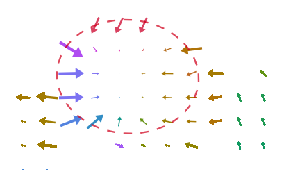
\includegraphics{spt/2_potential_well.eps}
  \caption{Example of a potential well in the velocity field obtained from the \tsc{SPT} data.}\label{fig:well}
\end{marginfigure}


\section{Regions of coherent motion}\label{sec:pathways}

We now study regions in the cell space where amyloid beta particles follow a coherently directed motion. The study of this kind of regions is not new in the literature and can find relevant applications in many biological contexts. As an example, coherent motion regions have been observed in interphase chromatin\mcite{zidovska2013}, yielding new hypothesis about chromatin biological functions. In our case, we would like to find out if Aβ is transported along well defined pathways.

We identified regions of coherent motion by clustering adjacent bins based on the angular distance of their  velocity vectors. The angular distance between two vectors $\bm{u}$ and $\bm{v}$ is defined as:
\begin{equation} \label{eq:angular-similarity}
 \mathrm{distance}(\bm{u}, \bm{v}) \equiv \frac{1}{\pi} \arccos\left(\frac{\bm{u} \cdot \bm{v}}{\|\bm{u}\| \|\bm{v}\|}\right)
\end{equation}

\noindent We adopted a very simple algorithm to perform the clustering:
\begin{enumerate}
 \begin{item}
       Create an empty cluster (i.e. a set of adjacent bins) for each bin in the grid and assign the bin to it.
\end{item}
\begin{item}
      For every bin $B$, consider each neighbouring bin $S \in \Gamma(B)$. If the angular distance between $\tilde{\bm{a}}(\bm{x}_B)$ and $\tilde{\bm{a}}(\bm{x}_S)$ is lower than a given threshold, merge the clusters of $B$ and $S$.
\end{item}
\end{enumerate}

\noindent This extremely simple method is quite effective in localising coherently directed motion. An example of the result is shown in \cref{fig:vf_cdr}.


\section{The full picture}\label{sec:full_picture}

In the previous sections we localised regions of attraction and pathways. One can hypothesise that the dynamics of Aβ is composite. Molecules may escape (by Brownian motion) from an attractor, then travel along a pathway and eventually drop into another attracting region. We considered this approach by connecting the regions of coherent motion and the potential wells to form a directed graph representing a rough dynamical map of the intracellular space.

First, the axis corresponding to the average direction of each region is computed; then the endpoints of the regions are connected to other endpoints or potential wells that are found in a small neighbourhood. The reconstructed structure is shown in \cref{fig:graph}.

Sadly, the results of this approach are a bit disappointing: the dynamical map that we were able to reconstruct by linking attractors and pathways is very complex and apparently meaningless.
\begin{figure}
  \sidecaption{Reconstruction of the dynamical structure. \subref{fig:graph_regions}\enskip coherent motion regions with main axis highlighted and attractors (in red), \subref{fig:graph_network}\enskip motion graph reconstructed by linking the regions of coherent motion and attractors.\label{fig:graph}}
  \includegraphics[width=\textwidth]{spt/graph.eps}
  {\phantomsubcaption{}\label{fig:graph_regions}}
  {\phantomsubcaption{}\label{fig:graph_network}}
\end{figure}
Although the methods to localise attractors and pathways described in \cref{sec:attractors,sec:pathways} were successful in their scope, the hope of identifying a global dynamics in the data seems vain. The analysis shows that there is no well defined pathway along which the Aβ aggregates are driven nor clear accumulation points. Instead, the molecules follow complex itineraries, bouncing between different regions. The reconstruction of the dynamical structure shown in \cref{fig:graph} gives an idea of the mess in the underlying motion. This leads us to formulate a new hypothesis. In fact, the behaviour may suggest that the processing of Aβ is highly delocalised, and molecules are bounced between several loosely distributed processing units. In the next chapter we will introduce a possible explanation for this behaviour, presenting a new model of motion and computing its characteristics.
